\section{Analytical Modeling}
In the previous section we studied the possibility of using a polynomial to capture the relationship between grain size, number of cores, and throughput for a fixed matrix size, with the purpose of finding a range of grain size that leads us to maximum performance. 
Although the polynomial function was helpful in directing us toward our objective, it does not have a physical implication. 

This motivated us to change our view, and instead of looking just at the data and trying to find a function to fit the data, study the behavior of the data, and then find a function that would be likely to fit the data. That function would be a good fit mostly because that's how we expect the throughput to change with grain size, and not just how the data looks like.   

In this chapter we attempt to understand the effect of grain size on the achievable speedup in an asynchronous many-task runtime system. As discussed in chapter~\ref{Background}, our knowledge here comes from Amdahl's law and Universal Scalibility Law, which is an extension to the Amdahl's law. What these models suggest is that as we increase the number of cores in a multicore system, we do not observe a linear speedup, and they hold two major factors accountable for that, latency.

Here we are interested in developing an analytical model for predicting the execution time in an asynchronous many task runtime system. Even if we were able to determine all the factors affecting the execution time, it is still very hard to find an analytical model describing the relationship between these factors and the execution time.   

Definitions:
We represent the overhead of creating one task with $\alpha$, the number of tasks created with $num\_{tasks}$, the maximum amount of work assigned to one core as $w\_c$, the number of cores that are actually doing the work as $M$, the total amount of work available as $problem\_{size}$, and the sequential execution time as $t_{seq}$.

In an attempt to find this analytical model, we started with looking into two major factors, the overhead of creating tasks, and the maximum amount of work assigned to one core. 
In order to understand how these factors contribute to the execution time, we created a benchmark based on a simple \textit{for\textunderscore{loop}} with different number of iterations, iteration lengths, and chunk sizes, as shown in Listing~\ref{hpx_for_loop}. 
Each iteration consists of a while loop that makes sure the iteration lasts a certain amount ot time. This way, knowing how long it would take to execute one iteration(denoted as \textit{iter\textunderscore{length}}), how many of iterations are executed by one HPX thread(denoted as \textit{chunk\textunderscore{size}}), and finally how many iterations there are(denoted as \textit{num\textunderscore{iterations}})), we can see how the execution time changes when the problem is executed on different number of cores. Here, we define \textit{problem\textunderscore{size}} as the time it takes to execute all the iterations, which is:

\begin{equation}\label{problem_size}
problem\_size = iter\_length\times{num\_iterations}
\end{equation}

The total execution time could be assumed to be the maximum amount of time it takes for one of the cores to finish it's work. With this assumption, the execution time for this simple problem, could be estimated as summation of maximum overhead of creating tasks on one core and the time it takes to run $w\_c$ amount of work on $N$ cores, shown in Formula~\ref{formula1}.

\begin{equation}\label{formula1}
execution\_time = \alpha\times\left \lceil{\frac{num\_{tasks}}{M}}\right \rceil +\:\:{(1+\gamma\times{(N-1)})\times{w\_c}}
\end{equation}
%\vspace{\baselineskip}

The first part of the equation is associated with the overhead of creating $num\_{tasks}$ tasks on $N$ cores, and the second part is deducted from the Universal Scalibilty Law\cite{gunther2007guerrilla}, that suggests there an overhead associated with the number of cores should be added to the expected execution time.

Figure shows an example of the results obtained from running the benchmark, for $problem\_size=10000$, on different number of cores.

\vspace{\baselineskip}	
\begin{figure}[H]
	\centering
	{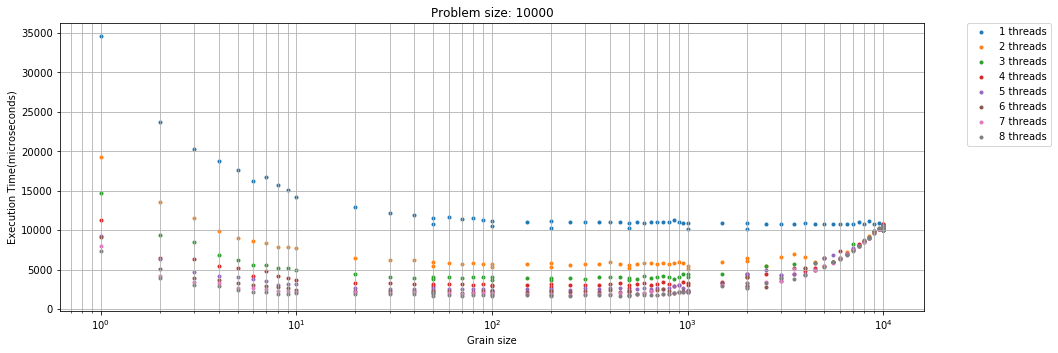
\includegraphics[scale=.45]{images/hpx_for_loop/10000_8_all.png}\label{fig29}}
	\caption{The results of running the benchmark in Listing with $problem\_size=10000$, on different number of cores.}		
\end{figure}

A stated in Chapter~\ref{Background}, at the left hand side of the graph in Figure~\ref{fig29},  the number of tasks created is smaller than the number of cores which results in making at least one of the cores idle, while the other cores are assigned a rather big chunk of work. The performance degradation we observe in that points is associated with starvation, meaning that we are not utilizing our computation resources to the full extent. In these points, the number of cores actually doing the work is equal to the number of the tasks, since each core gets to execute at most one task.    

To generalize the problem, assuming we are running our application on $N$ cores, with a grain size equal to $g$, $num\_{tasks}$ tasks are being created, and $M$ cores are actually doing the work. If $num\_{tasks}<N$, $M$ would be equal to $num\_{tasks}$, otherwise $M=N$.

%\begin{equation}
%M=\left\{
%\begin{aligned}
%num\_{tasks}\text{ if } num\_{tasks}<N\\
%N    \text{otherwise}
%\end{aligned}
%\right.
%\end{equation}


From overhead point of view though, if we represent the overhead of creating one task on a particular machine as $\alpha$, the overhead of creating $num\_{tasks}$ tasks would be $\alpha\times{num\_{tasks}}$, but this overhead is divided between the $M$ cores actually doing the work. 

%To summarize, knowing the grain size, we are expecting the execution time in a many-task runtime system to be mainly affected by these factors, the overhead of creating one task($\alpha$), the number of cores that are actually doing the work($M$), the sequential execution time($t_s$), and finally the portion of the program that could actually be parallelized($\gamma$). 
%
%If we try to integrate these information into a formula, we would expect the relation between execution time($t$) and number of tasks($n_t$) as follows:
%\begin{equation}\label{new1}
%t=\frac{\alpha{n_t}+t_s}{M}+\gamma
%\end{equation}
%
%which could be decomposed into these two equations:
%
%
%Now we use this function to find the best three parameters $\alpha$, $t_s$, and $\gamma$ so that the collected data would fit this model. For this purpose we used the \textit{curve\textunderscore{fit}} package from \textit{SciPy} library in \textit{python}.
%
%In order to make Equation~\ref{new1} differentiable, we used the softplus function(Equation~\ref{softplus1}) to represent $M$ based on $n_t$.
%\begin{equation}\label{softplus1}
%f(x)=Ln(1+e^x)
%\end{equation}
%
%Which results in Equation~\ref{soft_plus1}:
%\begin{equation}\label{soft_plus1}
%t=\frac{\alpha{n_t}+t_s}{(N-1)-Ln(1+(e^{N-1}-1)e^{-n_t})}+\gamma
%\end{equation}
%Throughout these experiments we try to fix or eliminate the factors we believe will affect the execution time as much as possible, study the results, and then introduce one factor to the model and study the behavior of the model. 
%\vspace{\baselineskip}

\begin{lstlisting}[basicstyle=\fontsize{8}{9}\selectfont,float,floatplacement=H,caption= {A simple hpx for\textunderscore{loop} used to study the effect of grain size on the achieved parallelism.}, label={hpx_for_loop}]

///////////////////////////////////////////////////////////////////////////////
void measure_function_futures_for_loop(std::uint64_t count, bool csv, std::uint64_t chunk_size, std::uint64_t iter_length)
{
// start the clock
high_resolution_timer walltime;
hpx::parallel::for_loop(hpx::parallel::execution::par.with(
hpx::parallel::execution::dynamic_chunk_size( chunk_size )),
0, count, [&](std::uint64_t) { worker_timed(iter_length*1000); });
// stop the clock
const double duration = walltime.elapsed();
print_stats("for_loop", "par", "parallel_executor", count, duration, csv);
}

///////////////////////////////////////////////////////////////////////////////
int hpx_main(variables_map& vm)
{
{
const int repetitions = vm["repetitions"].as<int>();
num_threads = hpx::get_num_worker_threads();
const std::uint64_t chunk_size = vm["chunk_size"].as<std::uint64_t>();
const std::uint64_t iter_length = vm["iter_length"].as<std::uint64_t>();
const std::uint64_t count = vm["num_iterations"].as<std::uint64_t>();
bool csv = vm.count("csv") != 0;
if (HPX_UNLIKELY(0 == count))
throw std::logic_error("error: count of 0 futures specified\n");
for (int i = 0; i < repetitions; i++)
{
measure_function_futures_for_loop(count, csv, chunk_size, iter_length);
}
}
return hpx::finalize();
}
///////////////////////////////////////////////////////////////////////////////
inline void worker_timed(std::uint64_t delay_ns)
{
if (delay_ns == 0)
return;
std::uint64_t start = hpx::util::high_resolution_clock::now();
while (true)
{
// Check if we've reached the specified delay.
if ((hpx::util::high_resolution_clock::now() - start) >= delay_ns)
break;chunk
}
}
///////////////////////////////////////////////////////////////////////////////
int main(int argc, char* argv[])
{
// Configure application-specific options.
options_description cmdline("usage: " HPX_APPLICATION_STRING " [options]");
cmdline.add_options()("num_iterations",
value<std::uint64_t>()->default_value(500000),
"number of iterations to invoke")
("repetitions", value<int>()->default_value(1),
"number of repetitions of the full benchmark")
("iter_length",value<std::uint64_t>()->default_value(1), "length of each iteration")
("chunk_size",value<std::uint64_t>()->default_value(1), "chunk size");
// Initialize and run HPX.
return init(cmdline, argc, argv);
}
\end{lstlisting}

For this simple experiment, where we do not have to deal with the cash effects, we believe the important factors are: number of HPX threads being created, number of cores the program is ran on, the maximum amount of work one core has to perform. The maximum number of tasks assigned to one core, and the number of cores that are actually performing the work, are two other important factors that can be deducted from the aforementioned factors. 

%\vspace{\baselineskip}
%\subsection{Step 1: Sequential Run}
%In the first step in order to eliminate all the factors related to parallel execution we run the code sequentially for some problem sizes. The obtained result, as shown in Figure~\ref{fig26} demonstrates an overhead that increases as the number of iterations increases.
%
%\begin{figure}
%	\centering
%	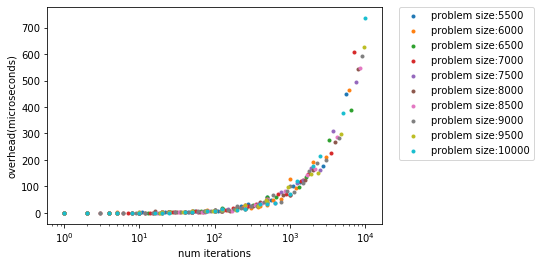
\includegraphics[width=1\linewidth]{images/hpx_for_loop/overheads_seq.png}
%	\caption{The results obtained from running the hpx for loop sequentially}	
%	\label{fig26}
%\end{figure}
%
%\subsection{Step 2: Single-task, single-core runs}
%At this step we look at the cases where only one task has been created, the program is run on only one core, and chunk size is set to one. This problem could be assumed to be equivalent to running the same amount of work sequentially with an additional cost of creating just one task. 
%
%\vspace{\baselineskip}
%\subsubsection{Expected Model}
%With this assumption we expect the execution time to be summation of the time it takes to perform the total amount of work(\textit{problem\textunderscore{size}}) and the overhead of creating one HPX task($\alpha$). Formula~\ref{chunk1} shows the expected formula.
%
%\begin{equation}\label{chunk1}
%execution\:\:time = \alpha + problem\:\:size
%\end{equation}  
%
%\vspace{\baselineskip}
%\subsubsection{Original Data}
%In order to check our proposed model for this simplified problem, we collected data from running the program, setting the \textit{chunk\textunderscore{size}} to 1, \textit{num\textunderscore{iterations}} to 1, and changing the \textit{iter\textunderscore{length}} from 1 to 10,000,000. 



\vspace{\baselineskip}